\documentclass{article}

% URLs and hyperlinks ---------------------------------------
\usepackage{hyperref}
\hypersetup{
	colorlinks=true,
	linkcolor=blue,
	filecolor=magenta,      
	urlcolor=blue,
}
\usepackage{xurl}
%---------------------------------------------------

\usepackage{graphicx}
\usepackage{rotating}
\usepackage{mathtools}
\usepackage{enumitem}

\usepackage{xepersian}
\settextfont{Yas}
\setdigitfont{Yas}

\title{
	گزارش کار آزمایش سوم \\ مدار معادل تونن و نورتون
}
\author{
	گروه: \\
	اریسا احسانی \\
	سید حسین حسینی \\
	مهدی حق‌وردی \\ \\
	شعبه شش
}
\date{}
\renewcommand{\arraystretch}{1.4}

\begin{document}
	\maketitle
	\tableofcontents
	\clearpage
	
	\section{مدار معادل تونن}
	
		با توجه به مدار رو‌به‌رو، به سوالات پاسخ دهید.
		\begin{center}
			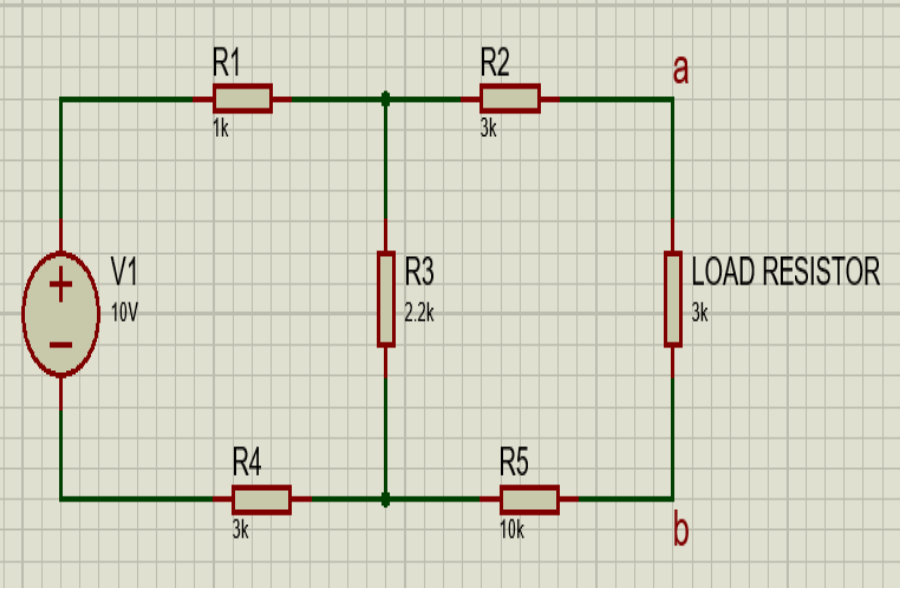
\includegraphics[width=11cm, height=6cm]{./images/R3.1.1}
		\end{center}
	
		\begin{enumerate}[label=\Alph*), align=left, leftmargin=*]
			\item 
			مقدار مقاومت تئوری ولتاژ‌ تونن را با پیدا کردن ولتاژ مدار باز بین دو نقطه‌ی \lr{a} و \lr{b} پیدا کنید.
			
			اختلاف ولتاژ دو نقطه‌ی 
			\lr{a}
			و
			\lr{b}
			را محاسبه می‌کنیم که برابر ولتاژ تونن 
			$\left(V_{\text{th}}\right)$
			خواهد بود.
			\begin{center}
				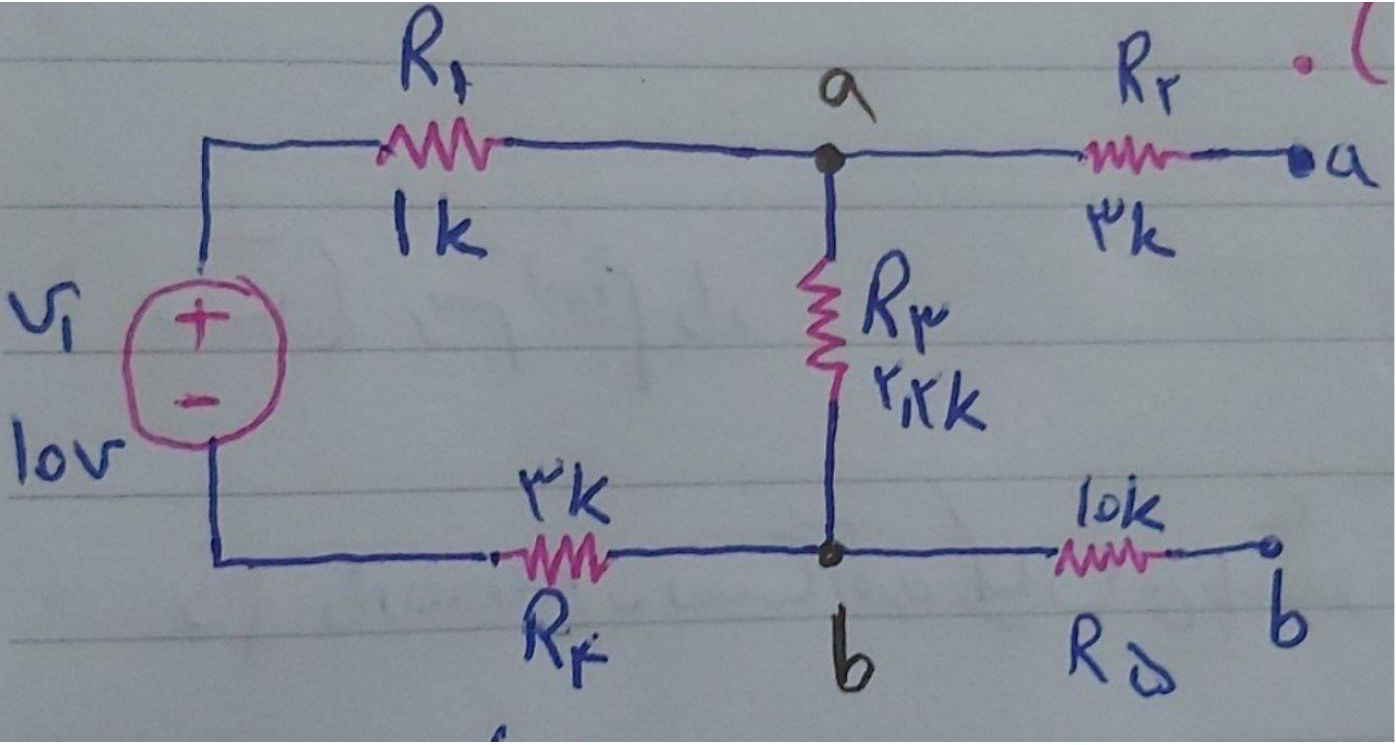
\includegraphics[width=11cm, height=8cm]{./images/R3.1.2}
			\end{center}
		
			مطابق مدار بالا، کافیست اختلاف ولتاژ دو سر مقاومت 
			$R_3$
			را محاسبه کنیم تا 
			$\left(V_{\text{th}}\right)$
			بدست بیاید.
			
			\begin{equation*}
				V_{\text{th}} = V_{R_{3}} = \frac{R_3}{R_3 + R_1 + R_4} \times V_1 = \frac{2.2 \times 10}{6.2} = 3.548 \, V
			\end{equation*}
			\item 
			سپس مقدار تئوری مقاومت تونن را با حذف مقاومت بار بدست آورید. (منبع ولتاژ $V_1$ را اتصال کوتاه کنید.)
			
			مقاومت تونن طبق شکل زیر بدست می‌آید.
			\begin{center}
				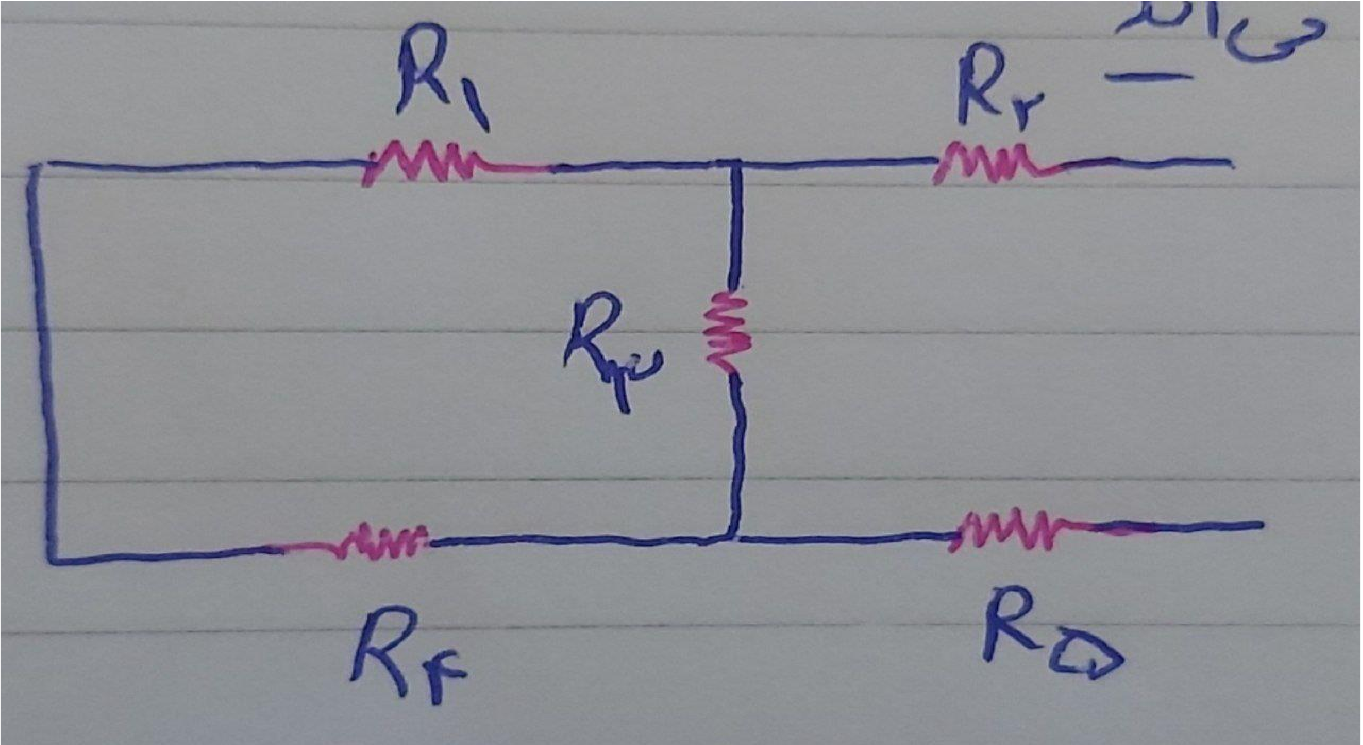
\includegraphics[width=11cm, height=8cm]{./images/R3.1.3}
			\end{center}
		
			\begin{equation*}
				R_{\text{th}} = \frac{R_3 \times (R_1 + R_4)}{R_3 + R_1 + R_4} + R_2 + R_5 = 14.419 \, K\Omega
			\end{equation*}
		
			\item 
			مدار معادل تونن را رسم کنید.
			\begin{center}
				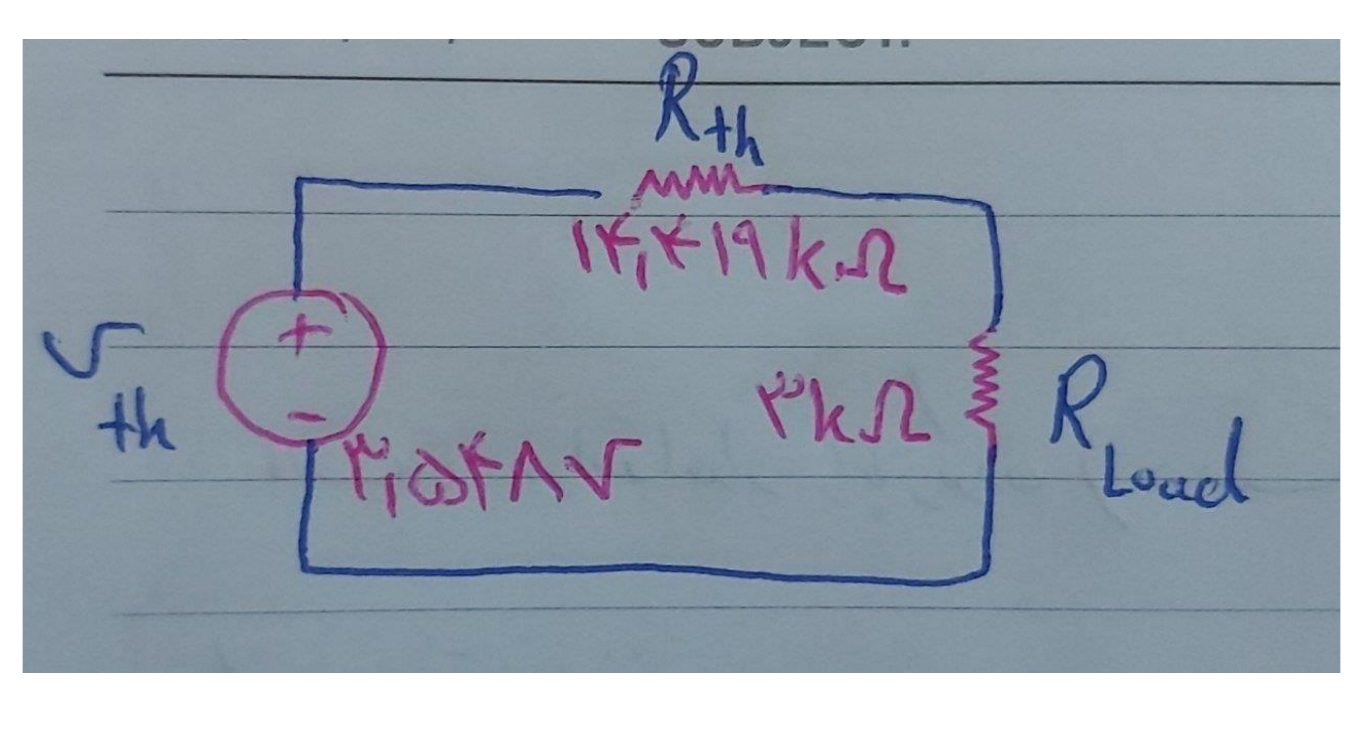
\includegraphics[width=11cm, height=8cm]{./images/R3.1.4}
			\end{center}
		
			\item 
			مدار بالا و مدار معادل تونن آن را، در نرم‌افزار شبیه‌سازی کنید. آیا ولتاژ مقاومت بار هر دو شبیه‌سازی، یک مقدار است؟ از نتیجه‌ی آن عکس بگیرید.
			
			\begin{center}
				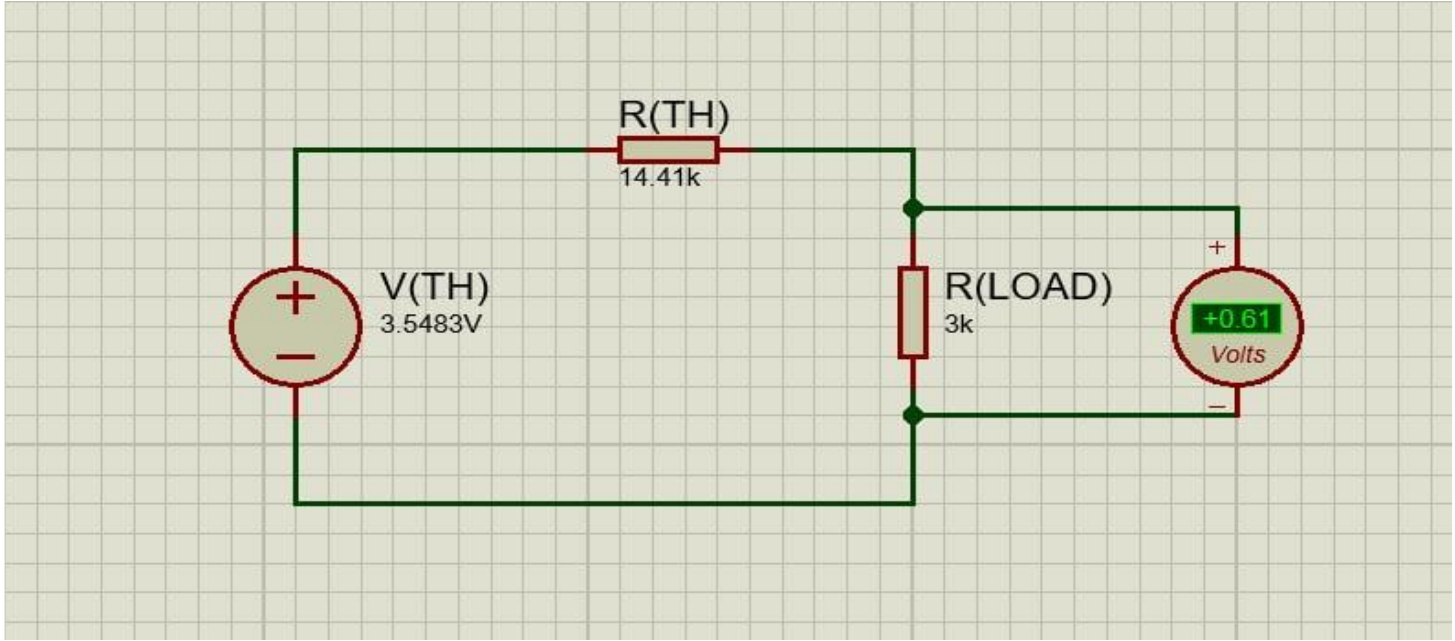
\includegraphics[width=11cm, height=6cm]{./images/R3.1.5}
			\end{center}
			\begin{center}
				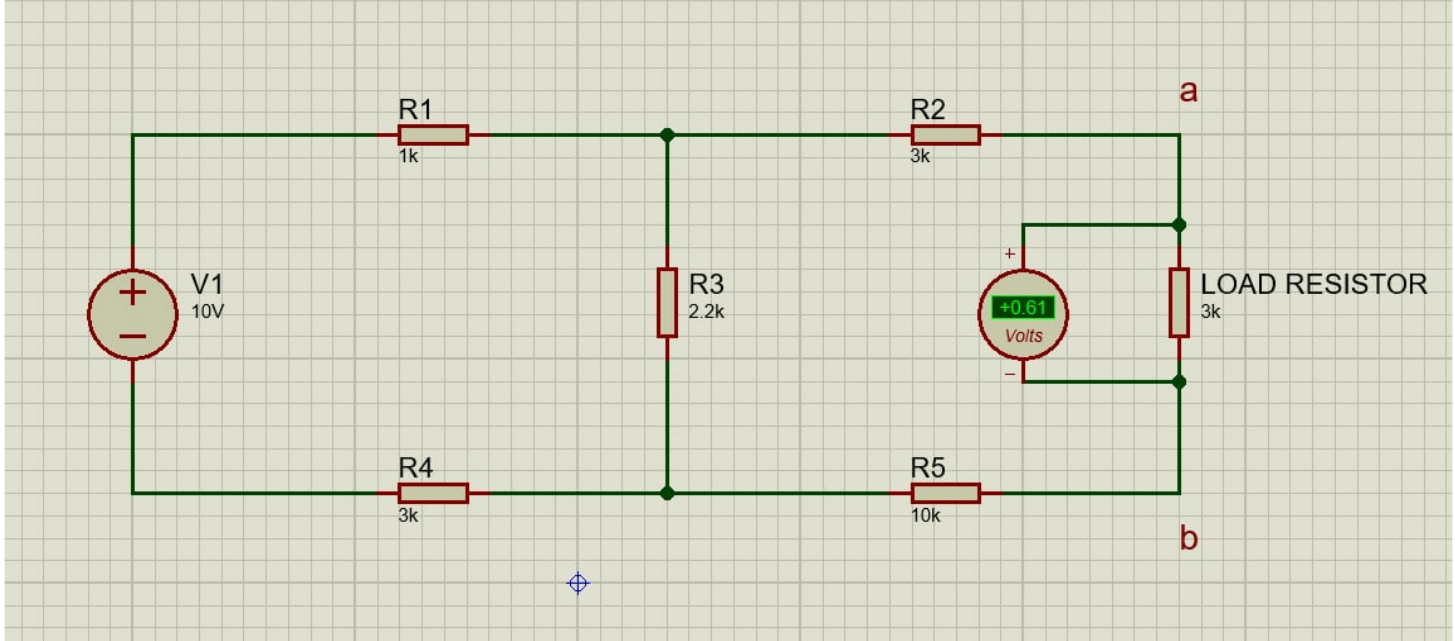
\includegraphics[width=11cm, height=6cm]{./images/R3.1.6}
			\end{center}
			
			مقادیر بدست‌ آمده، یکسان می‌باشند.
			
			\item 
			درصد خطای ولتاژ‌ مقاومت بار را نسبت به حالت تئوری اندازه‌گیری کنید.
			
			داده‌‌های بدست‌ آمده یکسان هستند و اختلاف جزئی ناشی از میزان دقت و خطای اعداد اعلام شده توسط ولت‌متر‌ها می‌باشد.
		\end{enumerate}
	
	\section{مدار معادل نورتون}
		\begin{enumerate}[label=\Alph*), align=left, leftmargin=*]
			\item 
			مقاومت نورتون را برای مدار قبل سوال قبل محاسبه کنید، رابطه‌ی آن با مقاومت تونن چگونه‌ است؟
			
			مقدار مقاومت نورتون با تونن برابر است و تفاوتی ندارد.
			
			\item 
			جریان نورتون را برای مدار سوال قبل محاسبه کنید.
			
			برای بدست آوردن 
			$I_{\text{sc}}$
			، دو سر مقاومت متصل به 
			\lr{a}
			و
			\lr{b}
			 را اتصال کوتاه کرده و جریان عبوری از 
			 \lr{a}
			 به
			 \lr{b}
			 را 
			 $I_{\text{sc}}$
			 می‌نامیم.
			 
			 \begin{center}
			 	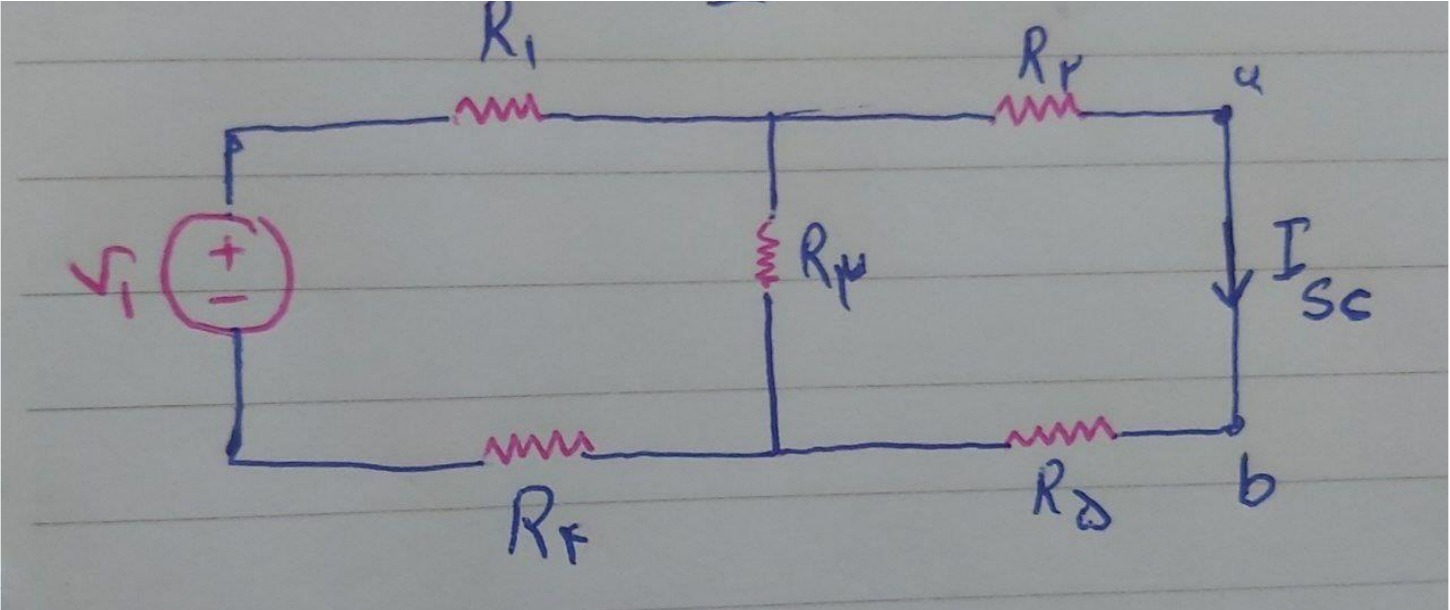
\includegraphics[width=11cm, height=5cm]{./images/R3.1}
			 \end{center}
			 
			 \begin{equation*}
			 	R_{\text{eq}} = \frac{R_3 \times (R_2 + R_5)}{R_3 + R_2 + R_5} + R_1 + R_4 = 5.8815 \, K\Omega 
			 \end{equation*}
		 
		 	\begin{equation*}
		 		I_{\text{total}} = \frac{V_1}{R_{\text{eq}}} = 1.7 \, mA
		 	\end{equation*}
	 	
	 		\begin{equation*}
	 			I_{\text{sc}} = \frac{R_3}{R_3 + R_2 + R_5} \times I_{\text{total}} = 0.246 \, mA
	 		\end{equation*}
 		
 			\begin{center}
 				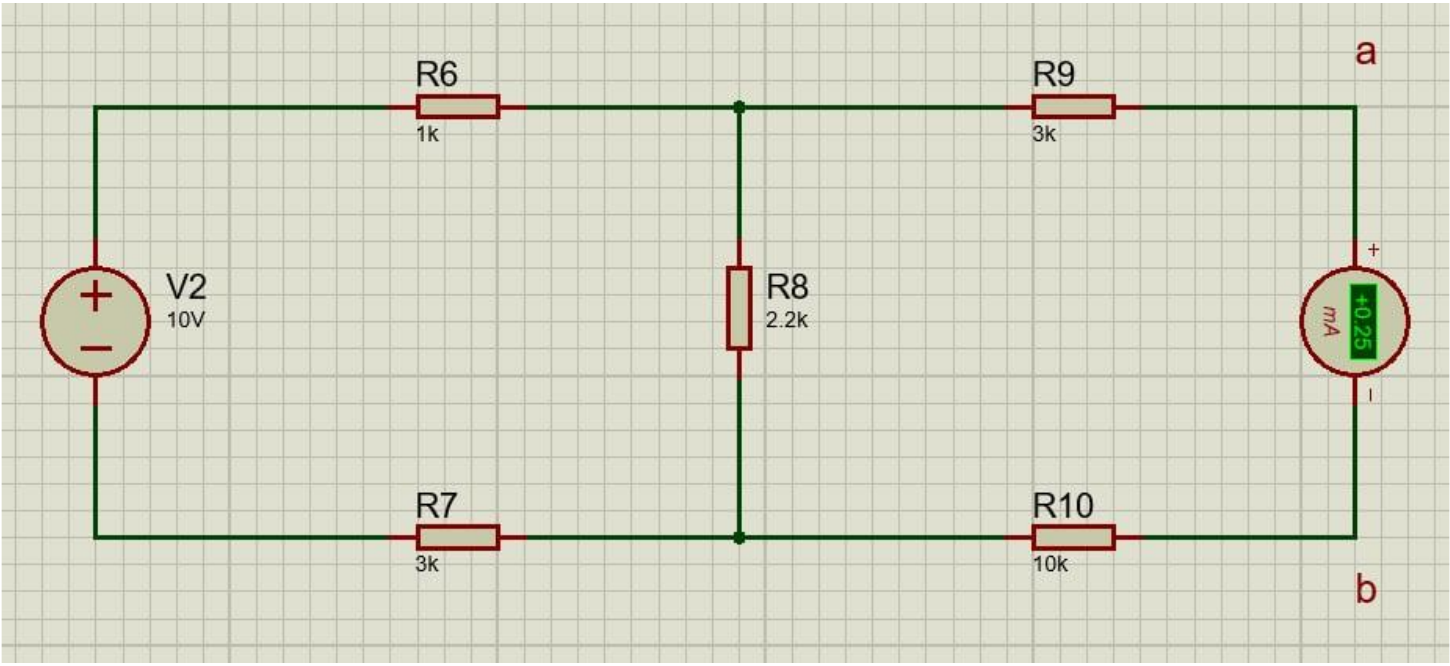
\includegraphics[width=11cm, height=6cm]{./images/R3.2}
 			\end{center}
 		
 		\item 
 		مدار معادل نورتون را برای مدار سوال قبل رسم کنید.
 		
 		\begin{center}
 			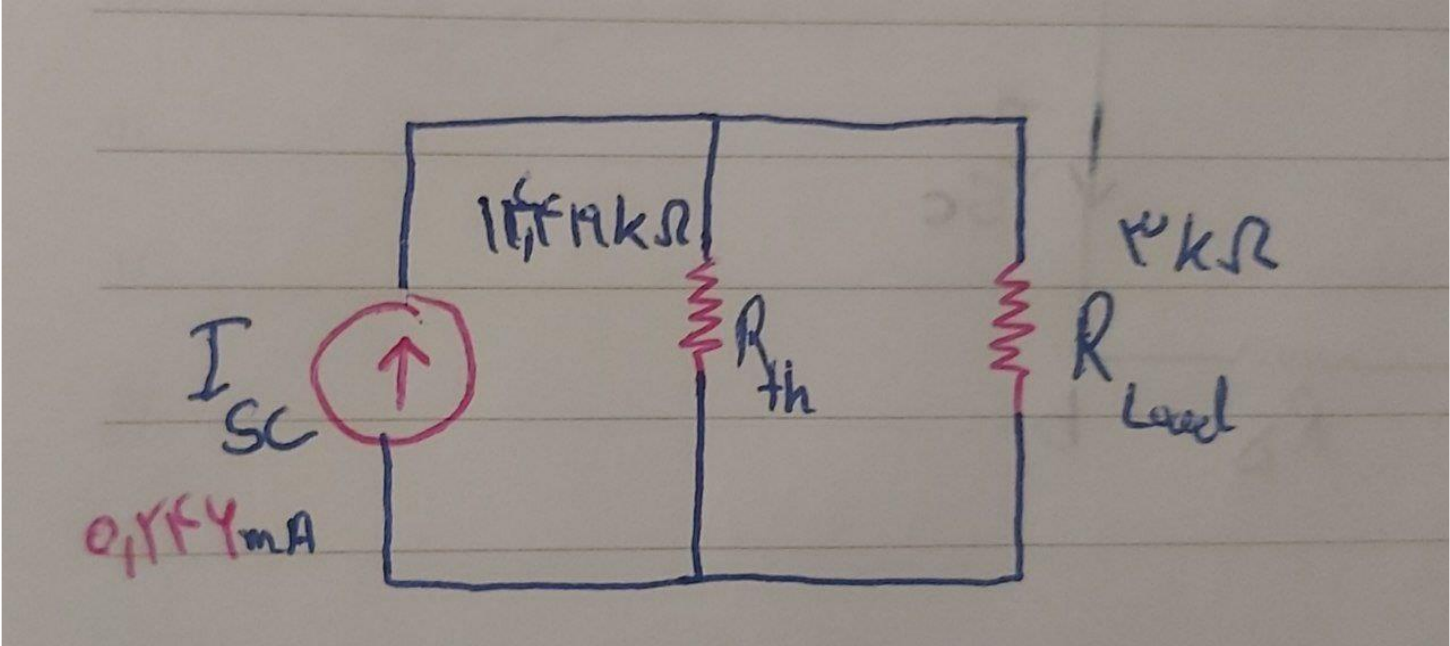
\includegraphics[width=11cm, height=6cm]{./images/R3.3}
 		\end{center}
 	
 		\item 
 			مدار بالا و معادل نورتون آن را در نرم‌افزار شبیه‌سازی کنید. آیا ولتاژ مقاومت بار هر دو شبیه‌سازی، یک مقدار است؟ از نتیجه‌هاتان عکس بگیرید.
 			
 			\begin{center}
 				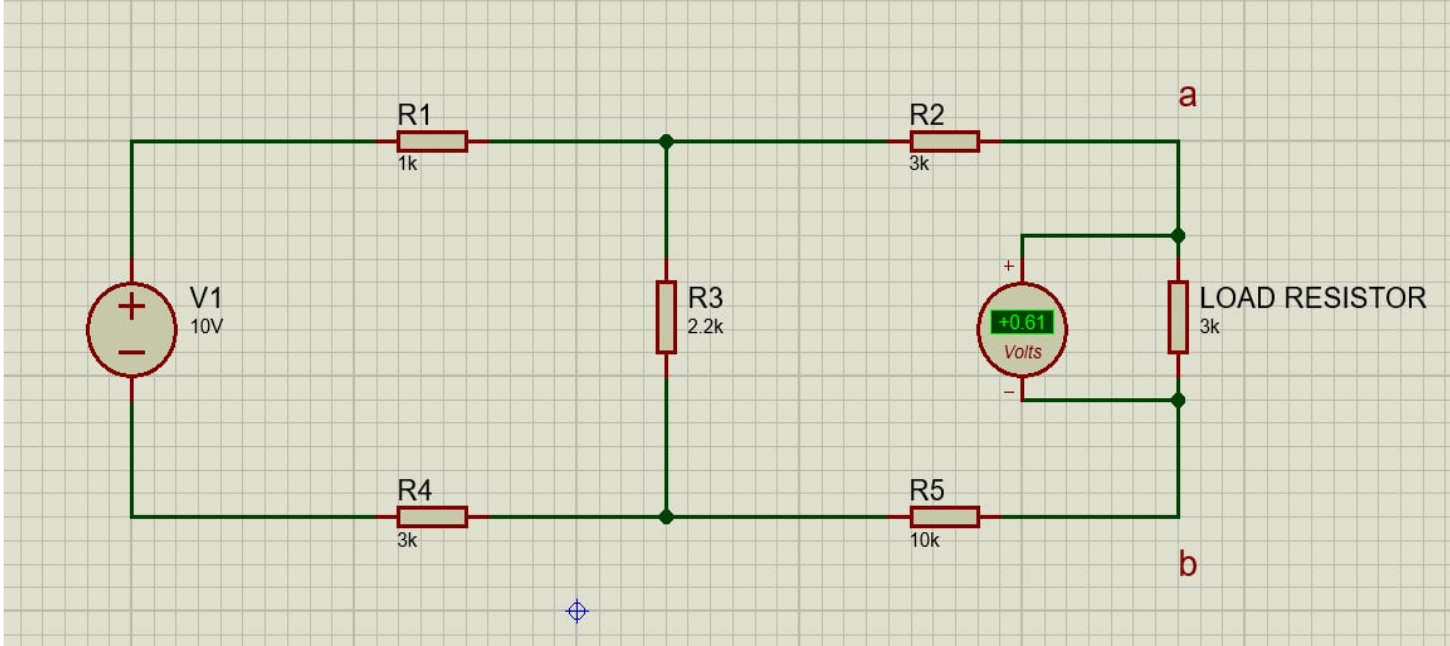
\includegraphics[width=11cm, height=6cm]{./images/R3.4}
 			\end{center}
 			\begin{center}
 				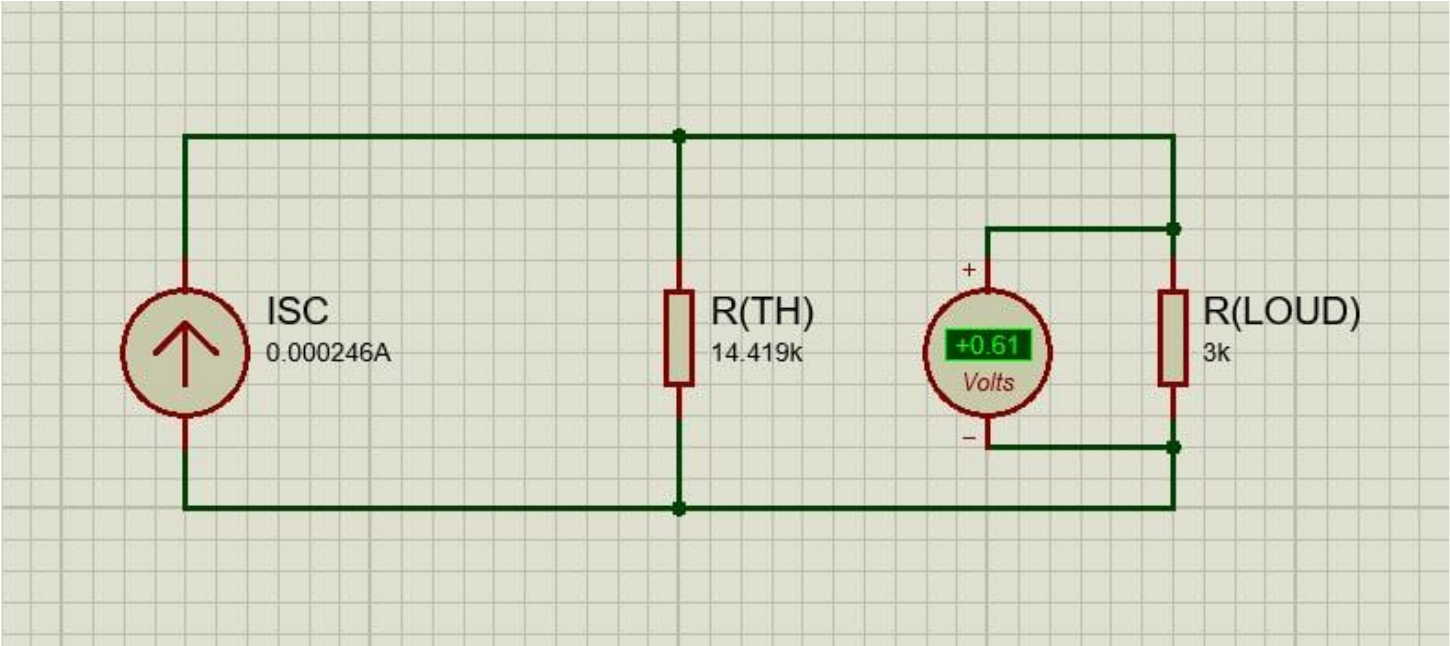
\includegraphics[width=11cm, height=6cm]{./images/R3.5}
 			\end{center}
 		
 		\item 
 		درصد خطای ولتاژ مقاومت بار را نسبت به حالت نئوری اندازه‌گیری کنید.
 		
 		داده‌‌های بدست‌ آمده یکسان هستند و اختلاف جزئی ناشی از میزان دقت و خطای اعداد اعلام شده توسط ولت‌متر‌ها می‌باشد.
 		
 		\item 
 		رایطه‌ی بین ولتاژی که اندازه‌گیری کردید با ولتاژ تونن چگونه است؟
 		
 		مقدار یکسانی دارند.
		\end{enumerate}
	
	\section{بیشترین توان مصرفی}
		مدار شکل داده شده را ببندید. در این مدار ولتاژ و مقامت تونن به این صورت است:
		
		\begin{center}
			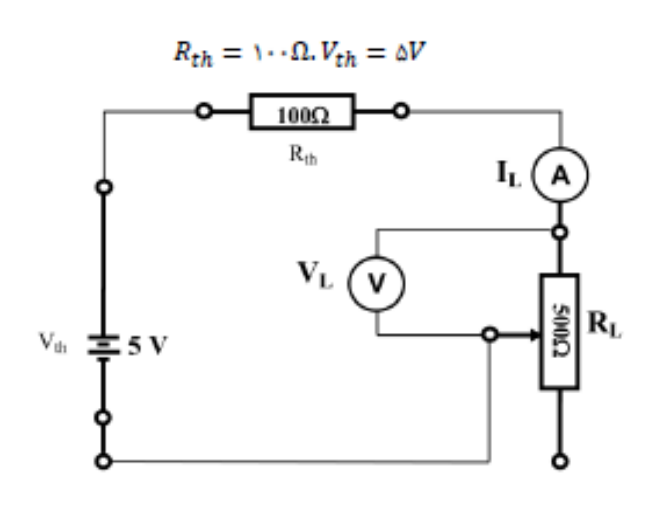
\includegraphics[width=8cm, height=8cm]{./images/R3.3.1}
		\end{center}
		
		\begin{table}[h]
			\begin{center}
				\begin{tabular}{|c|c|c|c|c|c|c|c|c|c|c|}
					\hline
					\multicolumn{11}{|c|}{$R_{\text{th}} = 100$} \\
					\hline
					\hline
					$300$ & $220$ & $180$ & $150$ & $120$ & $100$ & $80$ & $60$ & $40$ & $20$ & \lr{R} \\
					\hline
					\hline
					$0.02$ & $0.02$ & $0.02$ & $0.02$ & $0.03$ & $0.03$ & $0.03$ & $0.03$ & $0.04$ & $0.04$ & \lr{I} \\
					\hline
					\hline
					$3.00$ & $2.62$ & $2.37$ & $2.14$ & $1.87$ & $1.67$ & $1.43$ & $1.15$ & $0.83$ & $0.45$ & \lr{V} \\
					\hline
					\hline
					$0.06$ & $0.0525$ & $0.0474$ & $0.0428$ & $0.0561$ & $0.0501$ & $0.0429$ & $0.0345$ & $0.0332$ & $0.018$ & \lr{P} \\
					\hline
				\end{tabular}
			\end{center}			
		\end{table}
	
	\begin{table}[h]
		\begin{center}
			\begin{tabular}{|c|c|c|c|c|c|c|c|c|c|c|}
				\hline
				\multicolumn{11}{|c|}{$R_{\text{th}} = 150$} \\
				\hline
				\hline
				$300$ & $220$ & $180$ & $150$ & $120$ & $100$ & $80$ & $60$ & $40$ & $20$ & \lr{R} \\
				\hline
				\hline
				$0.01$ & $0.01$ & $0.02$ & $0.02$ & $0.02$ & $0.02$ & $0.02$ & $0.02$ & $0.02$ & $0.03$ & \lr{I} \\
				\hline
				\hline
				$1.50$ & $2.11$ & $1.87$ & $1.67$ & $1.43$ & $1.25$ & $1.05$ & $0.83$ & $0.59$ & $0.31$ & \lr{V} \\
				\hline
				\hline
				$0.0150$ & $0.0211$ & $0.0374$ & $0.0334$ & $0.0286$ & $0.0250$ & $0.0210$ & $0.0166$ & $0.0118$ & $0.0093$ & \lr{P} \\
				\hline
			\end{tabular}
		\end{center}			
	\end{table}
	
		نمودار توان بر حسب مقاومت بار را رسم کنید، و ماکزیمم توان را مشخص کنید.
		
		\begin{center}
			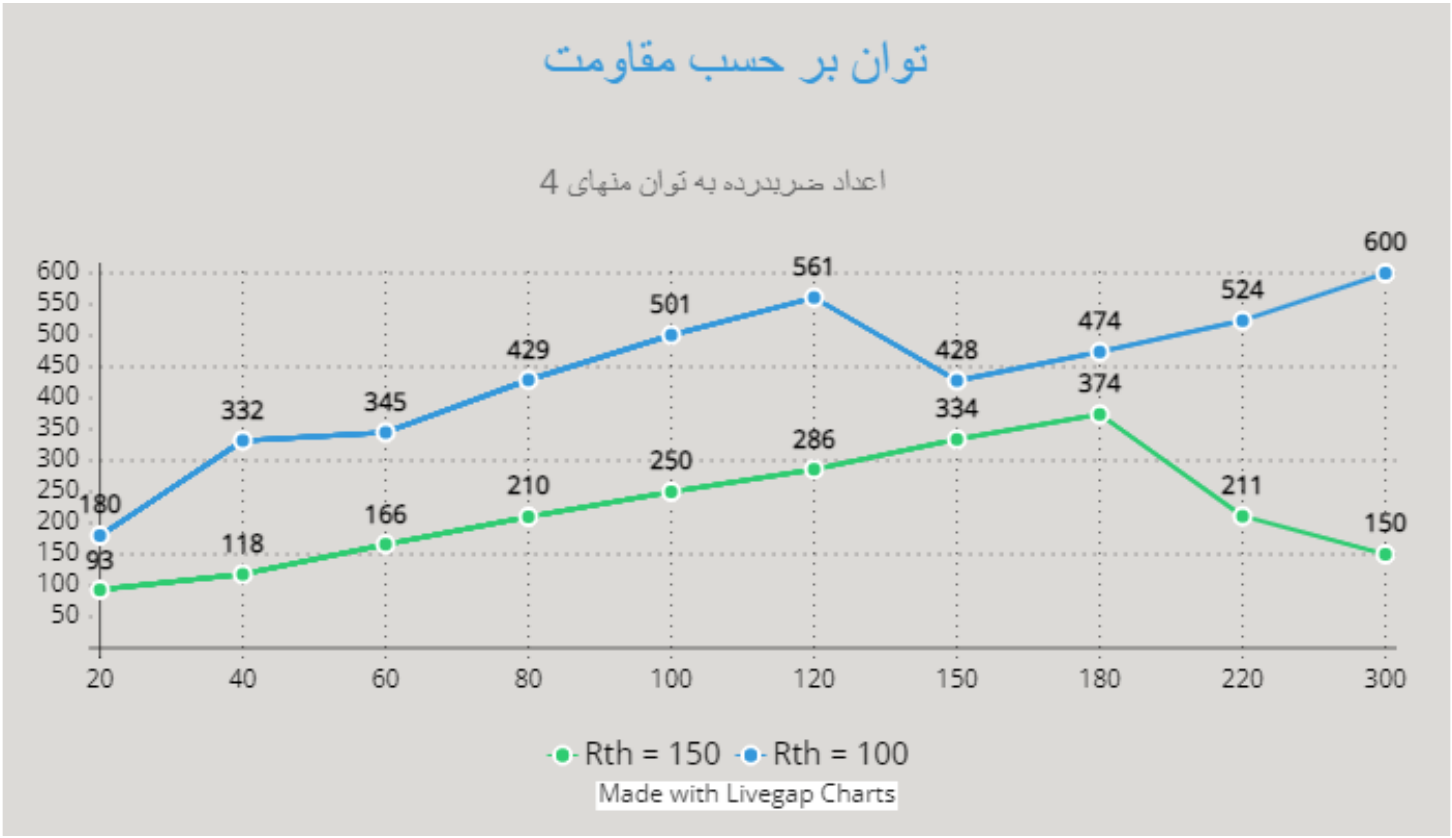
\includegraphics[width=13cm, height=10cm]{./images/R3.3.2}
		\end{center}
\end{document}
